\documentclass[conference]{IEEEtran}
\usepackage{amsmath,amssymb,amsfonts}
\usepackage{xcolor}
\usepackage{tikz}
\usetikzlibrary{patterns}
\usetikzlibrary{matrix}
\usepackage{pgfplots}
\pgfplotsset{compat=1.17}

\begin{document}

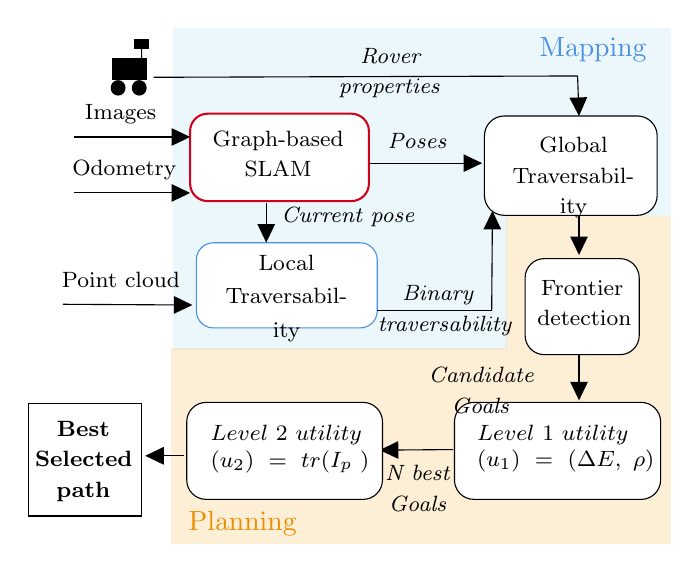
\begin{tikzpicture}[x=0.75pt,y=0.75pt,yscale=-1,xscale=1]

\draw  [draw opacity=0][fill={rgb, 255:red, 245; green, 166; blue, 35 }  ,fill opacity=0.19 ] (245.37,92.64) -- (324.67,92.64) -- (324.67,156) -- (245.37,156) -- cycle ;
\draw  [draw opacity=0][fill={rgb, 255:red, 80; green, 182; blue, 227 }  ,fill opacity=0.11 ] (245.67,2) -- (324.67,2) -- (324.67,92.64) -- (245.67,92.64) -- cycle ;
\draw  [draw opacity=0][fill={rgb, 255:red, 80; green, 182; blue, 227 }  ,fill opacity=0.11 ] (84.67,2) -- (245.67,2) -- (245.67,157) -- (84.67,157) -- cycle ;
\draw  [color={rgb, 255:red, 208; green, 2; blue, 27 }  ,draw opacity=1 ][fill={rgb, 255:red, 255; green, 255; blue, 255 }  ,fill opacity=1 ][line width=0.75]  (93,51.6) .. controls (93,46.95) and (96.77,43.18) .. (101.41,43.18) -- (170.72,43.18) .. controls (175.37,43.18) and (179.14,46.95) .. (179.14,51.6) -- (179.14,76.86) .. controls (179.14,81.51) and (175.37,85.28) .. (170.72,85.28) -- (101.41,85.28) .. controls (96.77,85.28) and (93,81.51) .. (93,76.86) -- cycle ;
\draw  [color={rgb, 255:red, 74; green, 144; blue, 226 }  ,draw opacity=1 ][fill={rgb, 255:red, 255; green, 255; blue, 255 }  ,fill opacity=1 ] (96,113.58) .. controls (96,109.06) and (99.67,105.38) .. (104.2,105.38) -- (174.94,105.38) .. controls (179.47,105.38) and (183.14,109.06) .. (183.14,113.58) -- (183.14,138.18) .. controls (183.14,142.71) and (179.47,146.38) .. (174.94,146.38) -- (104.2,146.38) .. controls (99.67,146.38) and (96,142.71) .. (96,138.18) -- cycle ;
\draw    (37,54.4) -- (90,54.4) ;
\draw [shift={(93,54.4)}, rotate = 180] [fill={rgb, 255:red, 0; green, 0; blue, 0 }  ][line width=0.08]  [draw opacity=0] (8.93,-4.29) -- (0,0) -- (8.93,4.29) -- cycle    ;
\draw    (37,81.36) -- (90,81.36) ;
\draw [shift={(93,81.36)}, rotate = 180] [fill={rgb, 255:red, 0; green, 0; blue, 0 }  ][line width=0.08]  [draw opacity=0] (8.93,-4.29) -- (0,0) -- (8.93,4.29) -- cycle    ;
\draw    (31.67,135) -- (91.12,135.34) ;
\draw [shift={(94.11,135.36)}, rotate = 180.33] [fill={rgb, 255:red, 0; green, 0; blue, 0 }  ][line width=0.08]  [draw opacity=0] (8.93,-4.29) -- (0,0) -- (8.93,4.29) -- cycle    ;
\draw    (129.67,86.18) -- (129.67,102.28) ;
\draw [shift={(129.67,105.28)}, rotate = 270] [fill={rgb, 255:red, 0; green, 0; blue, 0 }  ][line width=0.08]  [draw opacity=0] (8.93,-4.29) -- (0,0) -- (8.93,4.29) -- cycle    ;
\draw    (179.67,67) -- (230.67,67) ;
\draw [shift={(233.67,67)}, rotate = 180] [fill={rgb, 255:red, 0; green, 0; blue, 0 }  ][line width=0.08]  [draw opacity=0] (8.93,-4.29) -- (0,0) -- (8.93,4.29) -- cycle    ;
\draw    (238.29,138.18) -- (238.64,93) ;
\draw [shift={(238.67,90)}, rotate = 90.44] [fill={rgb, 255:red, 0; green, 0; blue, 0 }  ][line width=0.08]  [draw opacity=0] (8.93,-4.29) -- (0,0) -- (8.93,4.29) -- cycle    ;
\draw  [fill={rgb, 255:red, 255; green, 255; blue, 255 }  ,fill opacity=1 ] (234.8,53.85) .. controls (234.8,48.56) and (239.08,44.28) .. (244.37,44.28) -- (308.45,44.28) .. controls (313.73,44.28) and (318.02,48.56) .. (318.02,53.85) -- (318.02,82.57) .. controls (318.02,87.85) and (313.73,92.14) .. (308.45,92.14) -- (244.37,92.14) .. controls (239.08,92.14) and (234.8,87.85) .. (234.8,82.57) -- cycle ;
\draw    (183.14,138.18) -- (238.29,138.18) ;
\draw  [fill={rgb, 255:red, 0; green, 0; blue, 0 }  ,fill opacity=1 ] (55.51,16.67) -- (72.13,16.67) -- (72.13,26.75) -- (55.51,26.75) -- cycle ;
\draw  [fill={rgb, 255:red, 0; green, 0; blue, 0 }  ,fill opacity=1 ] (66.19,7.64) -- (73.15,7.64) -- (73.15,11.89) -- (66.19,11.89) -- cycle ;
\draw  [fill={rgb, 255:red, 0; green, 0; blue, 0 }  ,fill opacity=1 ] (55,30.73) .. controls (55,28.83) and (56.48,27.28) .. (58.31,27.28) .. controls (60.13,27.28) and (61.61,28.83) .. (61.61,30.73) .. controls (61.61,32.64) and (60.13,34.18) .. (58.31,34.18) .. controls (56.48,34.18) and (55,32.64) .. (55,30.73) -- cycle ;
\draw  [fill={rgb, 255:red, 0; green, 0; blue, 0 }  ,fill opacity=1 ] (65.18,30.73) .. controls (65.18,28.83) and (66.66,27.28) .. (68.48,27.28) .. controls (70.31,27.28) and (71.79,28.83) .. (71.79,30.73) .. controls (71.79,32.64) and (70.31,34.18) .. (68.48,34.18) .. controls (66.66,34.18) and (65.18,32.64) .. (65.18,30.73) -- cycle ;
\draw [fill={rgb, 255:red, 0; green, 0; blue, 0 }  ,fill opacity=1 ]   (69.67,9.77) -- (69.59,19.32) ;

\draw    (279.67,25) -- (280.26,41.28) ;
\draw [shift={(280.37,44.28)}, rotate = 267.92] [fill={rgb, 255:red, 0; green, 0; blue, 0 }  ][line width=0.08]  [draw opacity=0] (8.93,-4.29) -- (0,0) -- (8.93,4.29) -- cycle    ;
\draw    (280.37,92.28) -- (280.37,108.28) ;
\draw [shift={(280.37,111.28)}, rotate = 270] [fill={rgb, 255:red, 0; green, 0; blue, 0 }  ][line width=0.08]  [draw opacity=0] (8.93,-4.29) -- (0,0) -- (8.93,4.29) -- cycle    ;
\draw  [draw opacity=0][fill={rgb, 255:red, 245; green, 166; blue, 35 }  ,fill opacity=0.19 ] (83.67,156) -- (324.67,156) -- (324.67,250.28) -- (83.67,250.28) -- cycle ;
\draw  [fill={rgb, 255:red, 255; green, 255; blue, 255 }  ,fill opacity=1 ] (254.39,122.26) .. controls (254.39,117.14) and (258.54,113) .. (263.65,113) -- (300.11,113) .. controls (305.22,113) and (309.37,117.14) .. (309.37,122.26) -- (309.37,150.02) .. controls (309.37,155.13) and (305.22,159.28) .. (300.11,159.28) -- (263.65,159.28) .. controls (258.54,159.28) and (254.39,155.13) .. (254.39,150.02) -- cycle ;
\draw    (219.67,205) -- (187.37,205.25) ;
\draw [shift={(184.37,205.28)}, rotate = 359.55] [fill={rgb, 255:red, 0; green, 0; blue, 0 }  ][line width=0.08]  [draw opacity=0] (8.93,-4.29) -- (0,0) -- (8.93,4.29) -- cycle    ;
\draw  [fill={rgb, 255:red, 255; green, 255; blue, 255 }  ,fill opacity=1 ] (220.37,191.62) .. controls (220.37,186.46) and (224.55,182.28) .. (229.71,182.28) -- (310.32,182.28) .. controls (315.48,182.28) and (319.67,186.46) .. (319.67,191.62) -- (319.67,219.66) .. controls (319.67,224.82) and (315.48,229) .. (310.32,229) -- (229.71,229) .. controls (224.55,229) and (220.37,224.82) .. (220.37,219.66) -- cycle ;
\draw    (280.37,159.28) -- (280.37,178.28) ;
\draw [shift={(280.37,181.28)}, rotate = 270] [fill={rgb, 255:red, 0; green, 0; blue, 0 }  ][line width=0.08]  [draw opacity=0] (8.93,-4.29) -- (0,0) -- (8.93,4.29) -- cycle    ;
\draw  [fill={rgb, 255:red, 255; green, 255; blue, 255 }  ,fill opacity=1 ] (91.37,191.62) .. controls (91.37,186.46) and (95.55,182.28) .. (100.71,182.28) -- (176.32,182.28) .. controls (181.48,182.28) and (185.67,186.46) .. (185.67,191.62) -- (185.67,219.66) .. controls (185.67,224.82) and (181.48,229) .. (176.32,229) -- (100.71,229) .. controls (95.55,229) and (91.37,224.82) .. (91.37,219.66) -- cycle ;
\draw    (279.67,25) -- (75.37,25.64) ;
\draw    (90,208) -- (74.37,208) ;
\draw [shift={(71.37,208)}, rotate = 360] [fill={rgb, 255:red, 0; green, 0; blue, 0 }  ][line width=0.08]  [draw opacity=0] (8.93,-4.29) -- (0,0) -- (8.93,4.29) -- cycle    ;
\draw   (15,183) -- (69.67,183) -- (69.67,237) -- (15,237) -- cycle ;


% Text Node
\draw (41,37.4) node [anchor=north west][inner sep=0.75pt]  [font=\small] [align=left] {{\footnotesize Images}};
% Text Node
\draw (35,64.36) node [anchor=north west][inner sep=0.75pt]  [font=\small] [align=left] {{\footnotesize Odometry}};
% Text Node
\draw (30,118.36) node [anchor=north west][inner sep=0.75pt]  [font=\small] [align=left] {{\footnotesize Point cloud}};
% Text Node
\draw (186.88,51.5) node [anchor=north west][inner sep=0.75pt]  [font=\small] [align=left] {{\footnotesize \textit{Poses}}};
% Text Node
\draw (104.2,110.18) node [anchor=north west][inner sep=0.75pt]   [align=left] {\begin{minipage}[lt]{50.94pt}\setlength\topsep{0pt}
\begin{center}
{\footnotesize Local}
{\footnotesize Traversability}
\end{center}
\end{minipage}};
% Text Node
\draw (102.41,50.18) node [anchor=north west][inner sep=0.75pt]  [font=\small] [align=left] {\begin{minipage}[lt]{47.59pt}\setlength\topsep{0pt}
\begin{center}
{\footnotesize Graph-based }
{\footnotesize SLAM}
\end{center}

\end{minipage}};
% Text Node
\draw (245.72,53.32) node [anchor=north west][inner sep=0.75pt]  [font=\small] [align=left] {\begin{minipage}[lt]{46.08pt}\setlength\topsep{0pt}
\begin{center}
{\footnotesize Global}
{\footnotesize Traversability}
\end{center}
\end{minipage}};
% Text Node
\draw (150.14,10.28) node [anchor=north west][inner sep=0.75pt]  [font=\small] [align=left] {\begin{minipage}[lt]{56.97pt}\setlength\topsep{0pt}
\begin{center}
{\footnotesize \textit{Rover properties}}
\end{center}

\end{minipage}};
% Text Node
\draw (182.14,124.80) node [anchor=north west][inner sep=0.75pt]  [font=\small] [align=left] {\begin{minipage}[lt]{43.91pt}\setlength\topsep{0pt}
\begin{center}
{\footnotesize \textit{Binary }}\\{\footnotesize \textit{traversability}}
\end{center}

\end{minipage}};
% Text Node
\draw (260.14,5.28) node [anchor=north west][inner sep=0.75pt]  [color={rgb, 255:red, 74; green, 144; blue, 226 }  ,opacity=1 ] [align=left] {Mapping};
% Text Node
\draw (135.67,87.18) node [anchor=north west][inner sep=0.75pt]  [font=\small] [align=left] {{\footnotesize \textit{Current pose}}};
% Text Node
\draw (91,233.57) node [anchor=north west][inner sep=0.75pt]  [color={rgb, 255:red, 74; green, 144; blue, 226 }  ,opacity=1 ] [align=left] {\textcolor[rgb]{0.93,0.55,0.01}{Planning}};
% Text Node
\draw (184.37,211.28) node [anchor=north west][inner sep=0.75pt]  [font=\small] [align=left] {\begin{minipage}[lt]{25.97pt}\setlength\topsep{0pt}
\begin{center}
{\footnotesize \textit{N best }}\\{\footnotesize \textit{Goals}}
\end{center}

\end{minipage}};
% Text Node
\draw (258.99,122) node [anchor=north west][inner sep=0.75pt]  [font=\small] [align=left] {\begin{minipage}[lt]{32.51pt}\setlength\topsep{0pt}
\begin{center}
{\footnotesize Frontier }\\{\footnotesize detection}
\end{center}

\end{minipage}};
% Text Node
\draw (17,190) node [anchor=north west][inner sep=0.75pt]  [font=\small] [align=left] {\begin{minipage}[lt]{34.95pt}\setlength\topsep{0pt}
\begin{center}
{\footnotesize \textbf{Best }}\\{\footnotesize \textbf{Selected }}\\{\footnotesize \textbf{path}}
\end{center}

\end{minipage}};
% Text Node
\draw (223.37,190.28) node [anchor=north west][inner sep=0.75pt]  [font=\footnotesize]  {$ \begin{array}{l}
Level\ 1\ utility\ \\
( u_{1}) \ =\ ( \Delta E,\ \rho )
\end{array}$};
% Text Node
\draw (192.37,164.05) node [anchor=north west][inner sep=0.75pt]  [font=\small] [align=left] {\begin{minipage}[lt]{59.43pt}\setlength\topsep{0pt}
\begin{center}
{\footnotesize \textit{Candidate Goals }}
\end{center}

\end{minipage}};
% Text Node
\draw (94.99,190.68) node [anchor=north west][inner sep=0.75pt]  [font=\footnotesize]  {$ \begin{array}{l}
Level\ 2\ utility\ \\
( u_{2}) \ =\ tr( I_{p} \ )
\end{array}$};


\end{tikzpicture}

\end{document}